% Chapter 1

\chapter{Simulation Results} % Write in your own chapter title
\label{Chapter5}
\lhead{Chapter 5. \emph{Simulation Results}} % Write in your own chapter title to set the page header
\section{Switching frequency}
\begin{figure}[htbp]
	\centering
	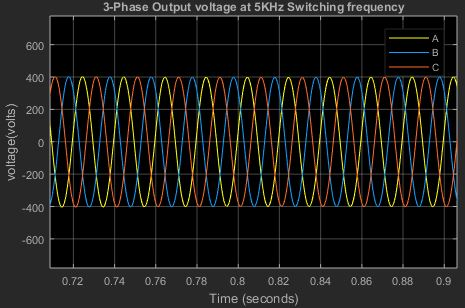
\includegraphics[width = 6in]{./Figures/5k.JPG}
	\rule{35em}{1pt}
	\caption{Output Volatge at 5KHz}
\end{figure}
\begin{figure}[htbp]
	\centering
	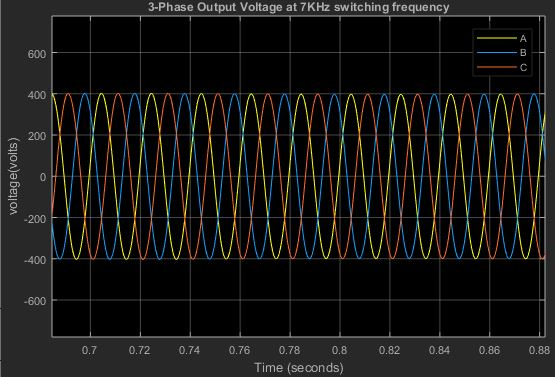
\includegraphics[width = 6in]{./Figures/7k.JPG}
	\rule{35em}{1pt}
	\caption{Output Volatge at 7KHz}
\end{figure}
\begin{figure}[htbp]
	\centering
	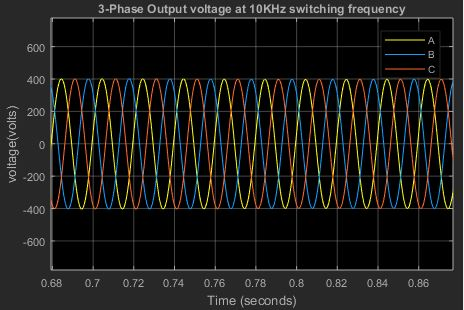
\includegraphics[width = 6in]{./Figures/10k.JPG}
	\rule{35em}{1pt}
	\caption{Output Volatge at 10KHz}
\end{figure}
\begin{figure}[htbp]
	\centering
	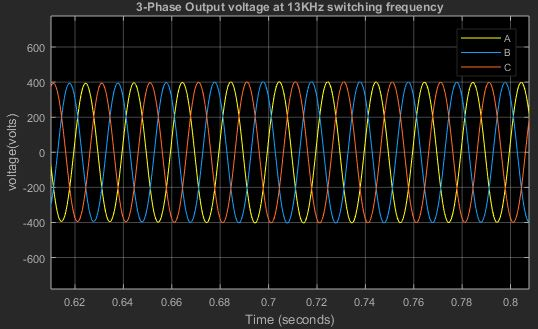
\includegraphics[width = 6in]{./Figures/13k.JPG}
	\rule{35em}{1pt}
	\caption{Output Volatge at 13KHz}
\end{figure}
\begin{figure}[htbp]
	\centering
	\includegraphics[width = 6in]{./Figures/15k.JPG}
	\rule{35em}{1pt}
	\caption{Output Volatge at 15KHz}
\end{figure}
\begin{figure}[htbp]
	\centering
	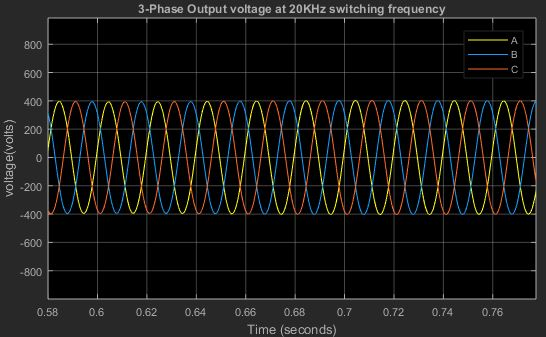
\includegraphics[width = 6in]{./Figures/20k.JPG}
	\rule{35em}{1pt}
	\caption{Output Volatge at 20KHz}
\end{figure}
\newpage
\section{Output at different rated value}
\begin{figure}[htbp]
	\centering
	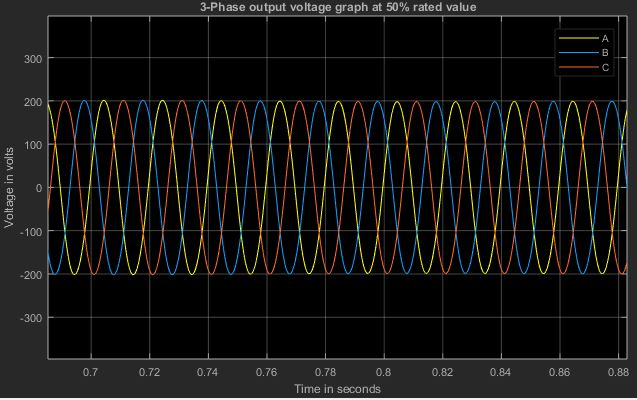
\includegraphics[width = 6in]{./Figures/50.JPG}
	\rule{35em}{1pt}
	\caption{Output Volatge at 50\% rated}
\end{figure}
\begin{figure}[htbp]
	\centering
	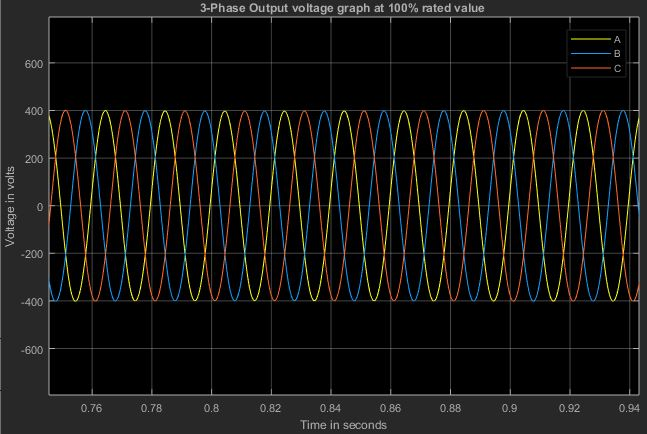
\includegraphics[width = 6in]{./Figures/100.JPG}
	\rule{35em}{1pt}
	\caption{Output Volatge at 100\% rated}
\end{figure}
\begin{figure}[htbp]
	\centering
	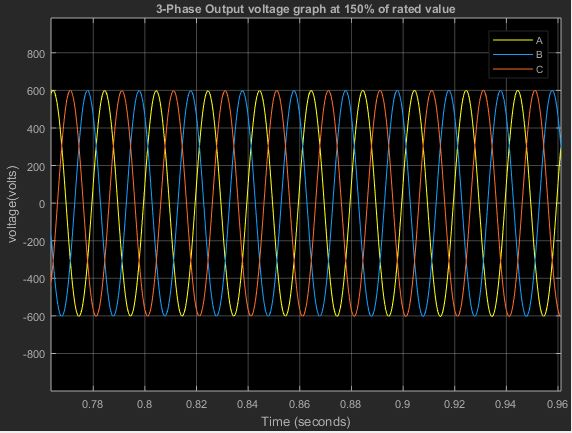
\includegraphics[width = 6in]{./Figures/150.JPG}
	\rule{35em}{1pt}
	\caption{Output Volatge at 150\% rated}
\end{figure}
\begin{figure}[htbp]
	\centering
	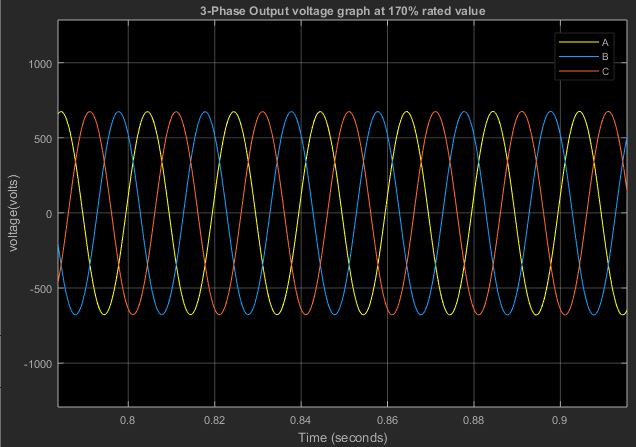
\includegraphics[width = 6in]{./Figures/170.JPG}
	\rule{35em}{1pt}
	\caption{Output Volatge at 170\% rated}
\end{figure}
\begin{figure}[htbp]
	\centering
	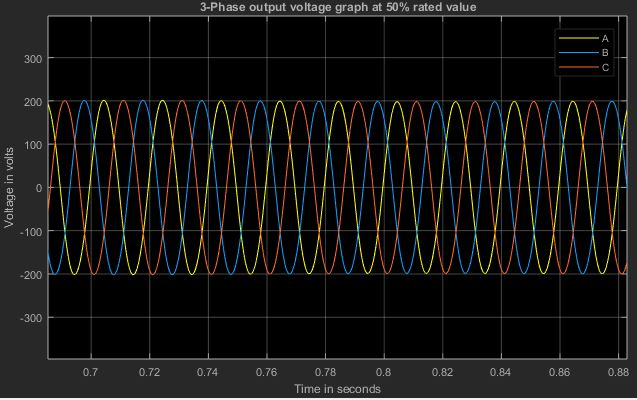
\includegraphics[width = 6in]{./Figures/50.JPG}
	\rule{35em}{1pt}
	\caption{Output Volatge at 50\% rated}
\end{figure}
\newpage
\subsection{Trend between Voltage and Index}
\begin{figure}[htbp]
	\centering
	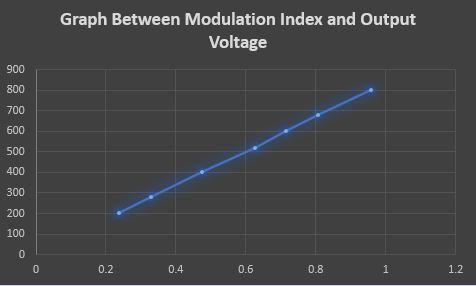
\includegraphics[width = 6in]{./Figures/mod.JPG}
	\rule{35em}{1pt}
	\caption{ModulationIndex and Output Volatge}
\end{figure}
\newpage
\section{Output Volatge at different frequencies}
\begin{figure}[htbp]
	\centering
	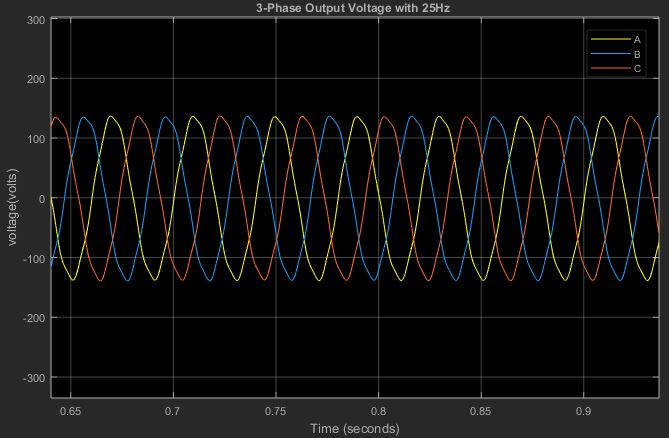
\includegraphics[width = 6in]{./Figures/25freq.JPG}
	\rule{35em}{1pt}
	\caption{Output Volatge Waveform at 25Hz}
\end{figure}
\begin{figure}[htbp]
	\centering
	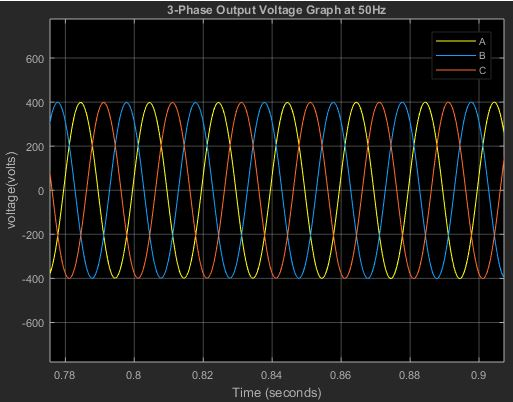
\includegraphics[width = 6in]{./Figures/50freq.JPG}
	\rule{35em}{1pt}
	\caption{Output Volatge Waveform at 50Hz}
\end{figure}
\begin{figure}[htbp]
	\centering
	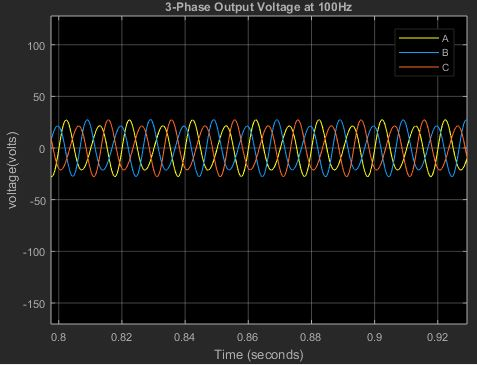
\includegraphics[width = 6in]{./Figures/100freq.JPG}
	\rule{35em}{1pt}
	\caption{Output Volatge Waveform at 100Hz}
\end{figure}
\subsection{Volatge and frequency trend}
\begin{figure}[htbp]
	\centering
	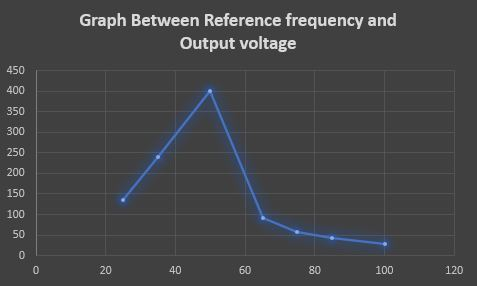
\includegraphics[width = 6in]{./Figures/graph2freq.JPG}
	\rule{35em}{1pt}
	\caption{Graph between ref. frequency and volatge}
\end{figure}
\begin{figure}[htbp]
	\centering
	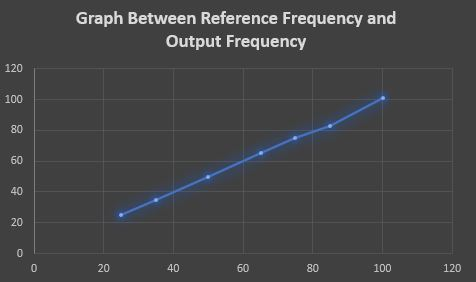
\includegraphics[width = 6in]{./Figures/graph1freq.JPG}
	\rule{35em}{1pt}
	\caption{Graph between ref. frequency and output frequency}
\end{figure}
\section{Task3}
Control the output voltage and frequency by using V/f principle. Discuss the limits of output
voltage and frequency that can be achieved. Reading is attached.
\begin{figure}[htbp]
	\centering
	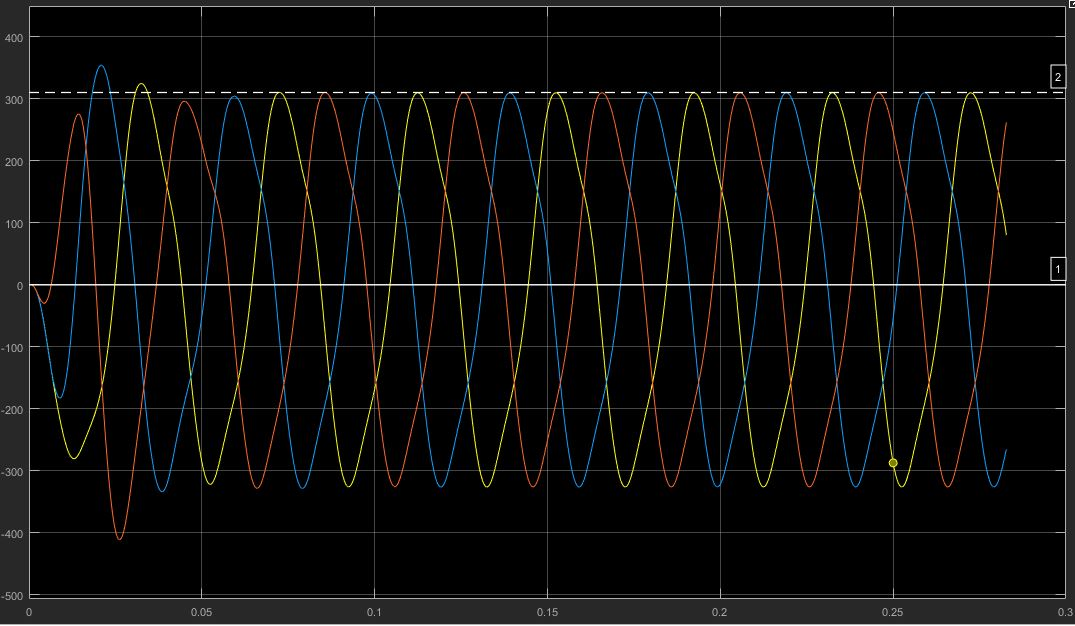
\includegraphics[width = 6in]{./Figures/Photos/task3/Task3_reading1/V313F25hz.JPG}
	\rule{35em}{1pt}
	\caption{Output volatage =313 and f = 25Hz}
\end{figure}
\begin{figure}[htbp]
	\centering
	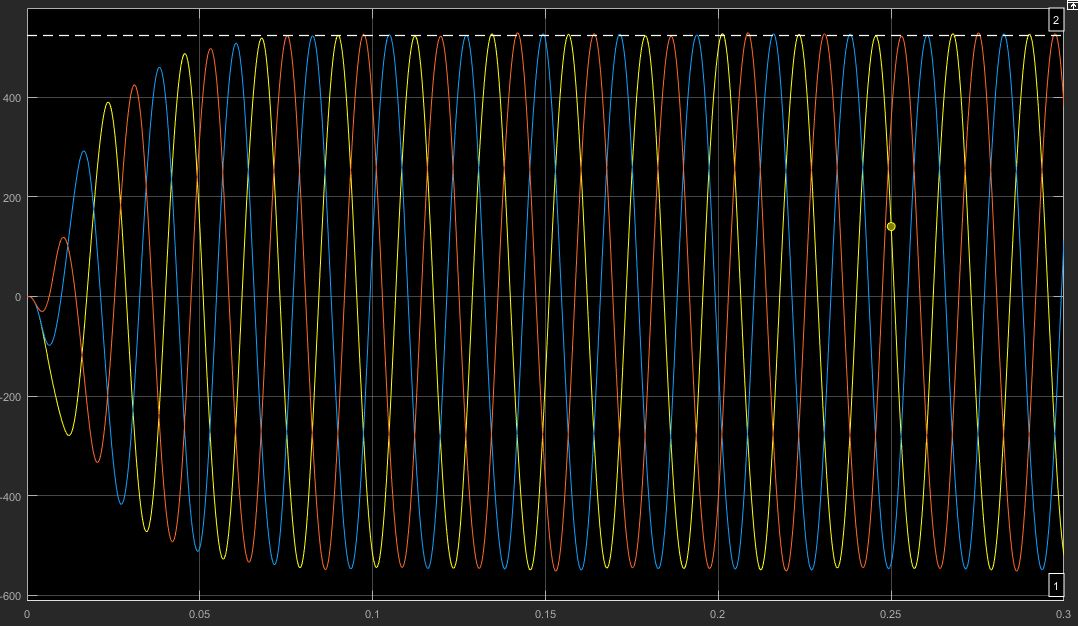
\includegraphics[width = 6in]{./Figures/Photos/task3/Task3_reading2/V525F45.JPG}
	\rule{35em}{1pt}
	\caption{Output volatage =525 and f = 45Hz}
\end{figure}
\begin{figure}[htbp]
	\centering
	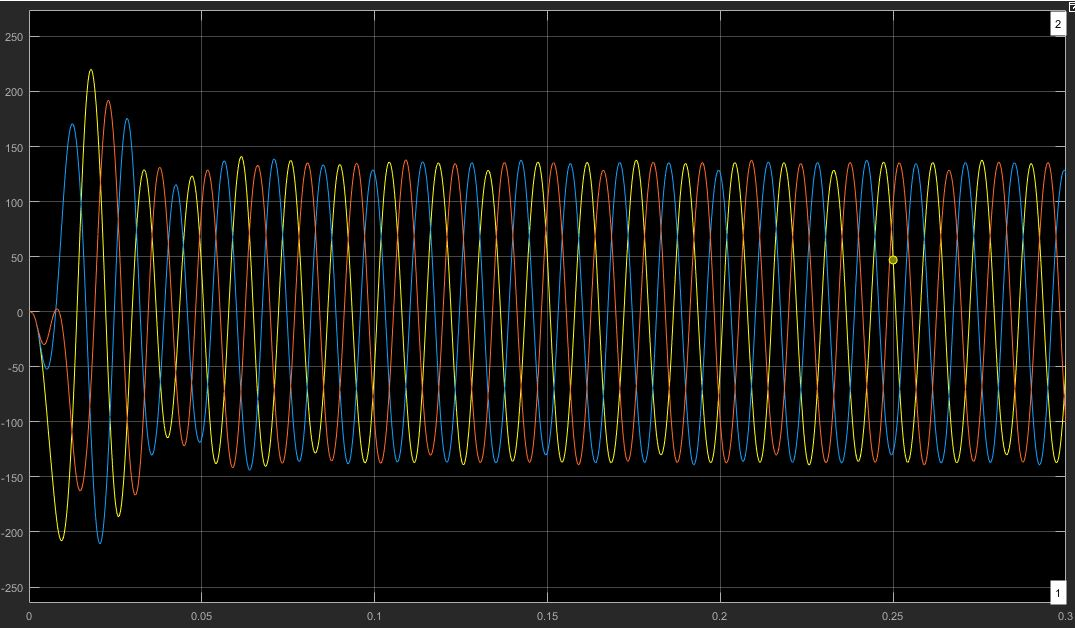
\includegraphics[width = 6in]{./Figures/Photos/task3/Task3_reading3/V132F70.JPG}
	\rule{35em}{1pt}
	\caption{Output volatage =132 and f = 70Hz}
\end{figure}
\subsection{frequency and volatge trend}
\begin{figure}[htbp]
	\centering
	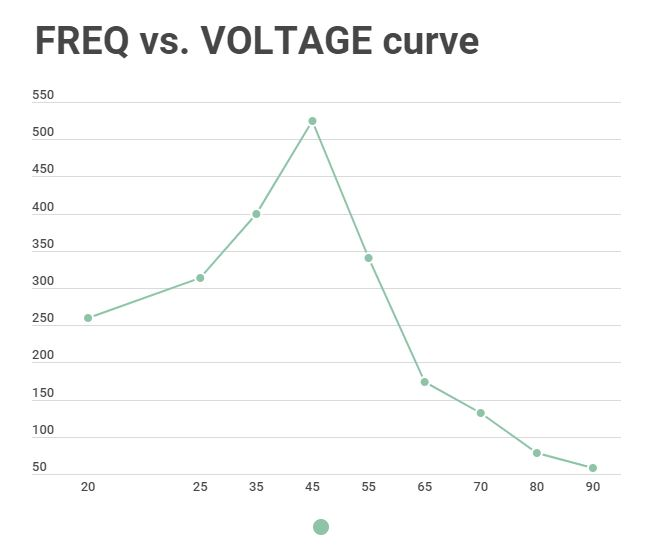
\includegraphics[width = 6in]{./Figures/Photos/task3/Graph1.JPG}
	\rule{35em}{1pt}
	\caption{trend for fixedV/f ration}
\end{figure}